\chapter{模擬データによる定量評価 \label{chapMock}}
% 3.1 模擬データの生成方法
% 3.2 解析方法
%  3.2.1 ベイズ推定の基礎
%  3.2.2 解析に用いる尤度関数
% 3.3 模擬データを用いた定量評価の結果
%  3.3.1 asymmetric driftの影響 (今、メールでは名称を省略しています)
%  3.3.2 ...影響
%  3.3.7 ...影響
% 3.4 解析結果のまとめ


% Chap. 3 模擬データ解析結果
% じっくり議論しながら整理したほうがよいので、
% また火曜日に議論しましょう。とりあえず、まだ書いていない 3.3.6、3.3.7も書いてみてください。


位置・速度の6次元位相空間観測データの模擬データを生成し、それを解析することで、asymmetric drift、視線速度の有無、速度楕円体の傾き、太陽からの距離$D$、円盤面からの距離$|z|$、データ数のそれぞれの解析への影響を定量的に評価した。この章ではそれらの結果についてまとめる。


\section{模擬データの生成方法}
観測方程式(\ref{ObsEq})に従う速度場を仮定し、密度分布には指数関数的密度分布$\rho(R,z) = \rho_0 e^{-R/h_R} e^{-z/h_z}、h_R=3\,\mathrm{kpc}、h_z=300\,\mathrm{pc}$\,(\cite{BH2016})を仮定している。ここで、$R,z$はそれぞれ円筒座標系での動径方向と鉛直方向の位置、$h_R、h_z$は$R、z$方向の密度分布のスケール長を示す。サンプル数は基本的に1000とし、太陽からの距離$D<1\,\mathrm{kpc}$としている。このときの3次元分布と1次元の頻度分布太陽の銀河中心からの距離は$R_{\odot} = 8.2\,\mathrm{kpc}$(\cite{BH2016})としている。また、asymmetric drift速度には式(\ref{AD3})を使用する。

%\subsection{模擬データの生成コード}
%以下に模擬データの作成コードのうちの1つを記述する。このコードではexponential diskを仮定し、太陽からの距離1kpc以内に1000個の星があるとしている。OLCODモデルに従った速度場を持たせている。
%\lstinputlisting[language=Python]{code/MockGenerate.py}

\begin{figure*}[htbp]
\begin{center}
	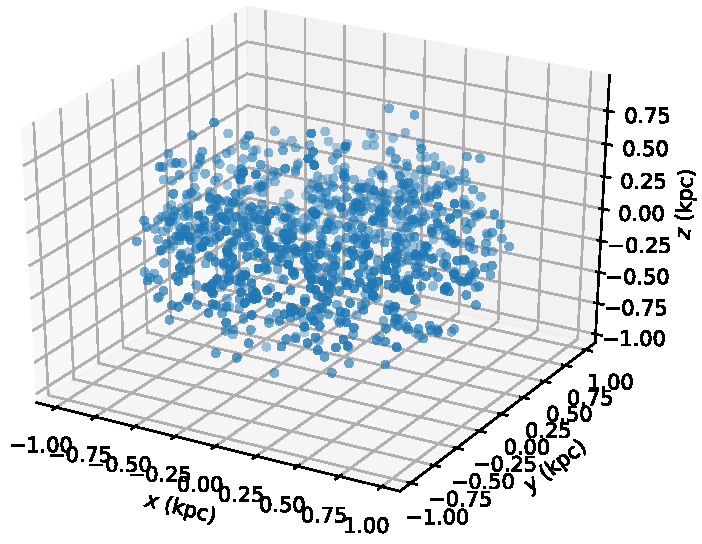
\includegraphics[width=9cm]{fig/3dMockData.pdf}
	\caption{1000個の星の模擬データの3次元分布} \label{dist3dMockData}
\end{center}
\end{figure*}

\begin{figure*}
   \centering
\begin{tabular}{ccc}
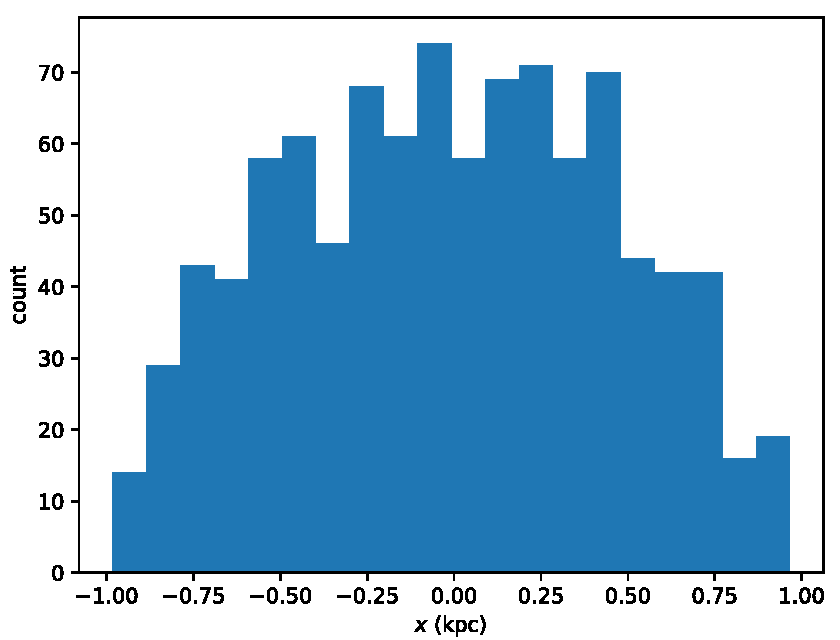
\includegraphics[width=4.5cm]{fig/dist_x.pdf}&
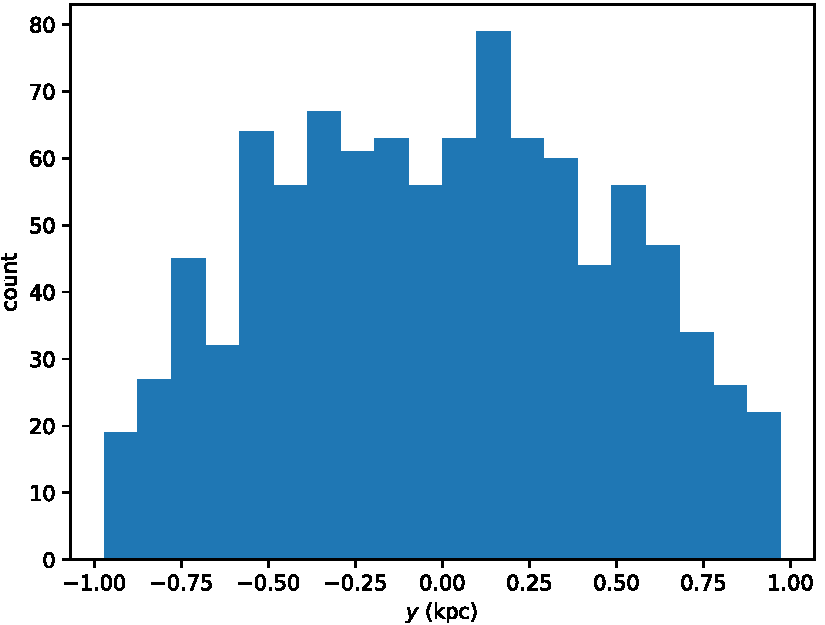
\includegraphics[width=4.5cm]{fig/dist_y.pdf}&
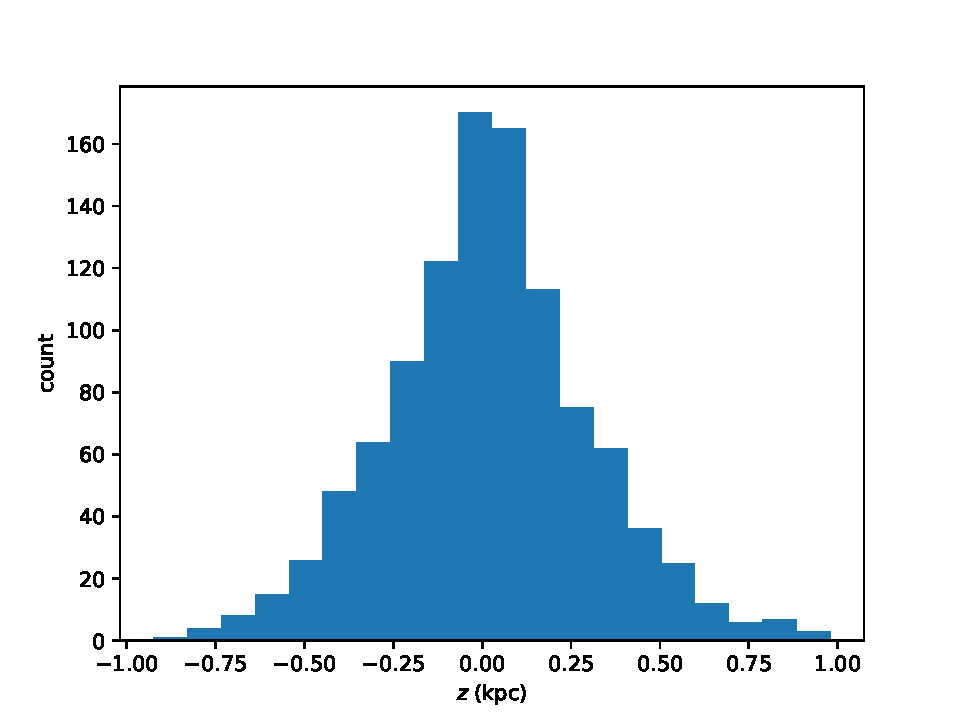
\includegraphics[width=4.5cm]{fig/dist_z.pdf}
\end{tabular}
    \caption{1000個の星の模擬データの頻度分布。$x、y、z$は太陽を支点とした直交座標系の軸の向きで、それぞれ銀河中心方向、銀河回転方向、銀河北極方向である。左の図から順に横軸は$x、y、z$、縦軸はそれぞれの値の範囲である。ビンは100 pcごとにしている。}
    \label{distMockData}
\end{figure*}

\begin{table}
\begin{center}
%\scalebox{0.5}
%\scriptsize
%\footnotesize
%\small
\begin{tabular}{c|c|c|c} \hline
 \rowcolor{LightCyan}
 星の年齢 $\tau\,\mathrm{(Gyr)}$ & $\sigma_R\,\mathrm{(km\ s^{-1})}$ & $\sigma_{\phi}\,\mathrm{(km\ s^{-1})}$ & $\sigma_{z}\,\mathrm{(km\ s^{-1})}$\\
 \hline
 1.4 & 21.7 & 12.0 & 8.6\\
 \hline
 1.9 & 21.4 & 16.7 & 10.1\\
 \hline
 2.4 & 27.8 & 18.9 & 10.5\\
 \hline
 2.8 & 32.7 & 18.4 & 11.0\\
 \hline
 3.3 & 31.3 & 16.8 & 11.9\\
 \hline
 3.8 & 30.1 & 16.9 & 11.7\\
 \hline
 4.3 & 34.7 & 17.8 & 12.6\\
 \hline
 4.9 & 36.8 & 21.2 & 16.8\\
 \hline
 5.6 & 39.3 & 22.1 & 17.7\\
 \hline
 6.4 & 42.5 & 23.0 & 18.3\\
 \hline
 7.2 & 43.8 & 24.2 & 23.3\\
 \hline
 8.5 & 51.8 & 25.8 & 23.3\\
 \hline
\end{tabular} \label{VelocityDispersion}
\vspace{3mm}
\caption{模擬データ生成で用いた年齢と速度分散の対応表 (\cite{YL18})。速度分散は銀河中心を中心とした円筒座標系$(R,\phi,z)$となっている。}
\end{center}
\end{table}

%%%%%%%%%%%%%%%%%%%%%%%%%%%%%%%%%%%%%%%%%%%%%%%%%%%%%%%%%%%%%%%%%%%%%%%%%%%%%%%%%%%%
%%%%%%%%%%%%%%%%%%%%%%%%%%%%%%%%%%%%%%%%%%%%%%%%%%%%%%%%%%%%%%%%%%%%%%%%%%%%%%%%%%%%

\section{解析方法}
この節では、第\ref{chapTheory}章を踏まえてデータの解析方法を説明する。まず本研究の解析で用いているベイズ推定について簡単に説明し、その後解析で使用している式や仮定について説明する。本論文では模擬データの生成と解析を7パターン行っており、それぞれの解析結果の詳細は\ref{模擬データの解析結果}で記述する。本節では、7パターンに共通する解析の基本的な部分を説明する。解析方法を大まかに分けると、asymmetric driftを考慮した場合と考慮しない場合とに分けられるため、この2パターンの解析方法については本節で説明する。

\subsection{ベイズ推定の基礎 \label{ベイズ推定の基礎}}
本研究では解析にベイズ推定(Bayesian Estimation)を用いる。ベイズ推定では、事後確率分布関数(Posterior probability distribution function; Posterior PDF)は事前確立分布関数(Prior PDF)、尤度関数(Likelihood function)を用いて次のように書ける。
\begin{align}
	事後確率分布関数 &= \frac{事前確率分布関数 \times 尤度関数}{観測値の分布関数} \\
			&\propto 事前確率分布関数 \times 尤度関数
\end{align}
事前確率分布とは、データが得られる前のある変数についての確率分布であり、事前確立分布関数は事前確率分布があるパラメータで書ける関数の形となっているものである。事後確率分布とは、事前確率分布にデータを入れた尤度関数を掛けて得られる分布であり、事後確立分布関数は事後確率分布があるパラメータで書ける関数の形となっているものである。尤度関数とは、あるデータが与えられたときに、そのデータの値の尤もらしさを出力する関数のことである。観測値の分布関数は確率の形に戻す(正規化する)ための定数と考えると、事前確率分布関数と尤度関数が重要なパラメータとなる。最尤推定法(Maximum Likelihood Estimation)は事前分布に一様分布を仮定しており尤度だけから真の値を推定するが、ベイズ推定では任意の事前分布をかけている。すると、$一様分布 \times 尤度関数$の確率分布の最頻値(尤度関数が最大の値)が最尤推定量となる。一方ベイズ推定では1つの値ではなく確率分布で与えられる。

ベイズ推定として最も広く使われる解析手法がマルコフ連鎖モンテカルロ法(Markov chain Monte Carlo methods; MCMC)である。マルコフ連鎖を利用したモンテカルロ法を用いると、データの分布を計算せずに直接事後分布を求めることができる。マルコフ連鎖(Markov chain)とは、ひとつのステップの中で前のパラメータの尤度に基づいて次のパラメータを決めることをいう。また一般に、乱数を用いた計算アルゴリズムをモンテカルロ法(Monte Carlo method)と呼ぶ(モンテカルロがカジノで有名なためにこう名付けられたという。ラスベガス法という別の方法も存在する)。

モンテカルロ法は、真にランダムにサンプリングを行うため
\begin{itemize}
	\item{計算コストがかさむ}
	\item{精度が向上しない}
\end{itemize}
という課題がある。計算コストがかさむ理由は、MCMCはマルコフ連鎖を利用していることから、限られた範囲で乱数発生をすればよいのに対し、モンテカルロ法のみの場合には毎ステップでマルコフ連鎖を利用する場合に比べて広範囲の乱数発生をしなくてはならず、その分計算コストが大きくなるためである。精度が向上しない理由は、マルコフ連鎖を利用しない場合には広範囲で乱数発生をしなければならないが、その際に乱数をあまり細かくすると計算コストが膨大になるため、広範囲な乱数を発生する代償として乱数は粗くなることになり、結果的に得られる確率分布の精度は悪くなる。MCMCは、マルコフ連鎖を定常分布としたサンプリングを行うことで、上記の課題を改善した方法である。

MCMCのアルゴリズムは以下の通りである。
\begin{enumerate}
	\item{初期点を決める}
	\item{マルコフ連鎖により次のサンプリングを行う分布を決定する}
	\item{分布が収束をするまで、(2)を繰り返す}
\end{enumerate}
基本的なアルゴリズムはこのようなものであるが、さらに具体的なアルゴリズムには高速化や精度の向上を目指していくつかの方法が開発されており、それらの一部に付録で触れることとする。本研究では、MCMCの解析に天文学研究で広く使われているemcee (\cite{Foreman2013}) を使用している。

%%%%%%%%%%%%%%%%%%%%%%%%%%%%%%%%%%%%%%%%%%%%%%%%%%%%%%%%%%%%%%%%%%%%%%%%%%%%%%%%%%%%
%%%%%%%%%%%%%%%%%%%%%%%%%%%%%%%%%%%%%%%%%%%%%%%%%%%%%%%%%%%%%%%%%%%%%%%%%%%%%%%%%%%%

\subsection{解析に用いる尤度関数 \label{解析に用いる尤度関数}}
MCMCによる解析では尤度関数を定義する必要がある。ここでは、本研究の解析で用いているフィッティングパラメータと尤度関数についての説明を行う。

\subsubsection{(a) asymmetric driftを考慮しない場合}
フィッティングパラメータは$A、B、C、K、U_{\odot}、V_{\odot}、W_{\odot}、\sigma_{\mu_l}、\sigma_{\mu_b}、\sigma_{v_{\mathrm{los}}}$の10個である。このときの尤度関数を求める。$\sigma_{\mu_l}、\sigma_{\mu_b}、\sigma_{v_{\mathrm{los}}}$はそれぞれ$\mu_l、\mu_b、v_{\mathrm{los}}$の平均速度場からの速度分散を表す。このとき尤度関数$\mathcal{L}$は
\begin{align}
\begin{aligned}
	\ln \mathcal{L} =& -\frac{1}{2}\sum_i \left(\frac{\left[\mu_{l,i} - \mu_l^{\mathrm{OL}}(l_i,b_i,\varpi_i)\right]^2}{\sigma_{\mu_l}^2 + (s_{\mu_{l,i}})^2}  + {\rm ln}\left[\sigma_{\mu_l}^2 + (s_{\mu_{l,i}})^2\right] \right. \\
	&+ \left. \frac{\left[\mu_{b,i} - \mu_b^{\mathrm{OL}}(l_i,b_i,\varpi_i)\right]^2}{\sigma_{\mu_b}^2 + (s_{\mu_{b,i}})^2}  + {\rm ln}\left[\sigma_{\mu_b}^2 + (s_{\mu_{b,i}})^2\right] \right. \\
	&+ \left. \frac{\left[v_{\mathrm{los},i} - v^{\mathrm{OL}}_{\mathrm{los}}(l_i,b_i,\varpi_i)\right]^2}{\sigma_{v_{\mathrm{los}}}^2 + (s_{v_{\mathrm{los},i}})^2} + {\rm ln}\left[\sigma_{v_{\mathrm{los}}}^2 + (s_{v_{\mathrm{los},i}})^2\right] \right)
\end{aligned} \label{Likelihood_Mock}
\end{align}
と書ける。ここで、添字の$i$は$i$番目の星の値であることを示し、この添字があるパラメータは観測量である。また、$s_{\mu_{l,i}}、s_{\mu_{b,i}}、s_{v_{\mathrm{los},i}}$はそれぞれ$\mu_{l,i},\mu_{b,i},v_{\mathrm{los},i}$の観測誤差である。

\subsubsection{(b) asymmetric driftを考慮する場合}
フィッティングパラメータは同様に$A、B、C、K、U_{\odot}、V_{\odot}、W_{\odot}、\sigma_{\mu_l}、\sigma_{\mu_b}、\sigma_{v_{\mathrm{los}}}$の10個である。まず、以下の式で解析の準備を行う。
\begin{align}
\begin{aligned}
	D_i &= \varpi_i^{-1},\\
	R_i &= \sqrt{D_i^2 + R_{\odot}^2 - 2D_iR_{\odot}\cos{l_i}},\\
	\sin{a_i} &= \dfrac{D_i}{R_i}\sin{l_i},\\
	\cos{a_i} &= \sqrt{1 - \sin^2{a_i}},
\end{aligned} \label{eq142}
\end{align}
$D_i、R_i、l_i、a_i$については図(\ref{coor_a})を参照。
\begin{figure*}[htbp]
	\centering
	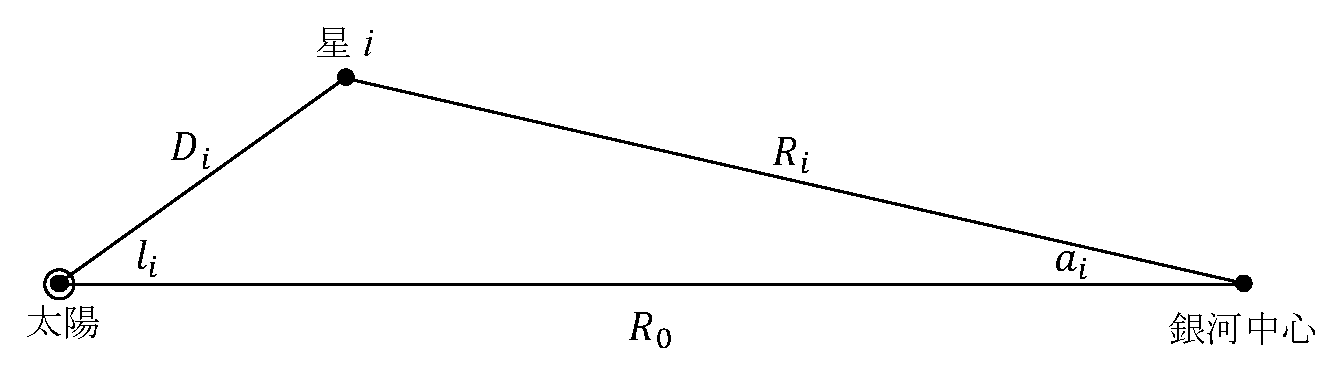
\includegraphics[width=10cm]{fig/coordinate_a2.pdf}
	\caption{星$i$と太陽、銀河中心の間のそれぞれの距離と角度の名称の定義。}
	\label{coor_a}
\end{figure*}
asymmetric driftを考慮するために、銀河中心に対する星と太陽の速度が必要となる。$v_R$の平均値$\overline{v_R}=0$という仮定を用いると、
\begin{align}
	v_{\mathrm{c}} = R_{\odot}(A-B) \label{eq153}
\end{align}
と表せる。また、接線速度は
\begin{align}
\begin{aligned}
	v_{l,i} =& \mu_{l,i}\varpi_i \kappa\\
	v_{b,i} =& \mu_{b,i}\varpi_i \kappa
\end{aligned}
\end{align}
と表せる。ここで、$\kappa=4.74047\,\si{km.s^{-1}.kpc^{-1}/(.mas.yr^{-1})}$は単位変換に用いられる定数である。円筒座標系の速度は
\begin{align}
\begin{aligned}
	\left(
	\begin{array}{c}
	 	v_{R,i}\\
		v_{\phi,i}\\
		v_{\mathrm{los},i}
	\end{array}
	\right)
	=& \bf{Q}^{\mathrm{T}} \left[\bf{P}^{\mathrm{T}}
	\left(
	\begin{array}{c}
	 	v_{l,i}\\
		v_{b,i}\\
		v_{\mathrm{los},i}
	\end{array}
	\right)
	+\left(
	\begin{array}{c}
	 	U_{\odot}\\
		V_{\odot} + v_{\mathrm{c}}\\
		W_{\odot}
	\end{array}
	\right)
	\right]
\end{aligned}
\end{align}
と変換される。ここから、$v_R$の標準偏差$\sigma_R$は
\begin{align}
\begin{aligned}
	\sigma_R =& \sqrt{\frac{1}{N}\sum^N_i(v_{R,i} - \overline{v_R})^2}
\end{aligned}
\end{align}
と計算できる。asymmetric drift速度は式(\ref{AD3})を採用する。。このasymmetric drift速度を銀河座標系に変換すると
\begin{align}
\begin{aligned}
	\left(
	\begin{array}{c}
	 	v_{a,l}\\
		v_{a,b}\\
		v_{a,\mathrm{los}}
	\end{array}
	\right)
	=& \bf{P} \bf{Q}
	\left(
	\begin{array}{c}
	 	0\\
		v_a\\
		0
	\end{array}
	\right)
\end{aligned}
\end{align}
のようになる。表記法は\ref{sec_ObsAD}と同様である。このとき尤度関数$\mathcal{L}$は
\begin{align}
\begin{aligned}
	\ln \mathcal{L} =& -\frac{1}{2}\sum_i \left(\frac{\left[\mu_{l,i} - \mu_l^{\mathrm{AD}}(l_i,b_i,\varpi_i)\right]^2}{\sigma_{\mu_l}^2 + (s_{\mu_{l,i}})^2}  + {\rm ln}\left[\sigma_{\mu_l}^2 + (s_{\mu_{l,i}})^2\right] \right. \\
	&+ \left. \frac{\left[\mu_{b,i} - \mu_b^{\mathrm{AD}}(l_i,b_i,\varpi_i)\right]^2}{\sigma_{\mu_b}^2 + (s_{\mu_{b,i}})^2}  + {\rm ln}\left[\sigma_{\mu_b}^2 + (s_{\mu_{b,i}})^2\right] \right. \\
	&+ \left. \frac{\left[v_{\mathrm{los},i} - v^{\mathrm{AD}}_{\mathrm{los}}(l_i,b_i,\varpi_i)\right]^2}{\sigma_{v_{\mathrm{los}}}^2 + (s_{v_{\mathrm{los},i}})^2} + {\rm ln}\left[\sigma_{v_{\mathrm{los}}}^2 + (s_{v_{\mathrm{los},i}})^2\right] \right)
\end{aligned}
\end{align}
と書ける。ここで、添字の$i$は$i$番目の星の値であることを示し、この添字があるパラメータは観測量である。ADの添字が付いているモデルの式については式(\ref{ObsEqAD})を参照。

%%%%%%%%%%%%%%%%%%%%%%%%%%%%%%%%%%%%%%%%%%%%%%%%%%%%%%%%%%%%%%%%%%%%%%%%%%%%%%%%
%%%%%%%%%%%%%%%%%%%%%%%%%%%%%%%%%%%%%%%%%%%%%%%%%%%%%%%%%%%%%%%%%%%%%%%%%%%%%%%%
%%%%%%%%%%%%%%%%%%%%%%%%%%%%%%%%%%%%%%%%%%%%%%%%%%%%%%%%%%%%%%%%%%%%%%%%%%%%%%%%

\section{模擬データの解析結果 \label{模擬データの解析結果}}
模擬データの解析では表\ref{table5}で書いているようにasymmetric drift、視線速度の有無、速度楕円体の傾き、太陽からの距離、円盤面からの距離、サンプル数、太陽の銀河中心からの距離$R_{\odot}$の7つの効果を考える解析パターンで、模擬データ生成あるいは解析方法を変更してオールト解析における7つの効果を調べた。表\ref{table4}、\ref{table5}はそれぞれの解析で用いた模擬データの設定と仮定を示している。asymmetric driftについては解析に際して入れる必要がある場合のみ模擬データに入れている。また、太陽は円盤面上に位置していると仮定している。$R_{\odot}$の効果を調べる理由は、先行研究で使われている$R_{\odot}$の値がだいたい$\SI{7.5}{kpc}$から$\SI{8.5}{kpc}$の間でばらつきがあり一定ではないため、仮定する$R_{\odot}$の値が解析に大きな影響を及ぼさないかどうか調べたいためである。

表\ref{table5}で試行回数について書いているが、この場合の試行回数とはすなわち模擬データ1を生成してそれを解析する、模擬データ2を生成してそれをまた解析する、という風に、試行回数が例えば10の場合には模擬データ1から模擬データ10までの10個の模擬データを生成してそれぞれを全く同様に解析するという意味である。最終的な解析結果には、試行回数分の結果の値の平均値を使用する。解析6以外の解析ではサンプル数は全て1000としている。これは、1000個のサンプルならばある程度の精度が得られ、かつ計算時間も長すぎないという都合からである。なお、1000サンプルでも各解析結果の評価にポアソンノイズが影響してしまうため、模擬データを模擬データ1、模擬データ2のように10個生成し、それぞれを解析して10個の解析結果の平均値を使用している。

また、それぞれの解析結果で各パラメータの相対誤差fit-trueと絶対誤差$\log_{10}\left| \dfrac{\mathrm{fit} - \mathrm{true}}{\mathrm{true}}\right|$をプロットしているが、相対誤差の絶対値の大きさの順番と絶対誤差の大きさの順番は必ずしも一致しない。なぜなら、相対誤差を計算するときには試行回数分の解析ごとの相対誤差を足しているので、例えばtrueの値が1の場合に試行1の相対誤差が1で試行2の相対誤差が-1だった場合でこの2回の平均値を考えると、相対誤差は$[1+(-1)]/2=0$となる一方、絶対誤差は$[|1|+|-1|]/2=1$となり、複数の解析結果の平均値を使用しているために相対誤差の絶対値をとったものが絶対誤差になる訳ではない。

\begin{table}
\begin{center}
%\scalebox{0.5}
%\scriptsize
%\footnotesize
%\small
\begin{tabular}{l|c} \hline
 \rowcolor{LightCyan}
 パラメータ & 値\\
 \hline
 $A$ & 18 $\mathrm{km\,s^{-1} kpc^{-1}}$\\
 \hline
 $B$ & -11 $\mathrm{km\,s^{-1} kpc^{-1}}$\\
 \hline
 $C$ & -2 $\mathrm{km\,s^{-1} kpc^{-1}}$\\
 \hline
 $K$ & -1 $\mathrm{km\,s^{-1} kpc^{-1}}$\\
 \hline
 $U_{\odot}$ & 9 $\mathrm{km\,s^{-1}}$\\
 \hline
 $V_{\odot}$ & 11 $\mathrm{km\,s^{-1}}$\\
 \hline
 $W_{\odot}$ & 7.5 $\mathrm{km\,s^{-1}}$\\
 \hline
 $R_{\odot}$ & 8.2 $\mathrm{kpc}$\\
 \hline
\end{tabular}
\vspace{3mm}
\caption{模擬データ生成で用いた各パラメータの設定値。}
\label{table4}
\end{center}
\end{table}



\begin{table}
\begin{center}
%\scalebox{0.5}
%\scriptsize
%\footnotesize
%\small
\begin{tabular}{l|c|c} \hline
 \rowcolor{LightCyan}
 解析名 & asymmetric drift & 試行回数 \\
 \hline
 解析1: asymmetric driftの解析結果への影響 & 有 & 3\\
 \hline
 解析2: 視線速度の有無による解析結果への影響 & 無 & 10\\
 \hline
 解析3: 速度楕円体の傾きの解析結果への影響 & 無 & 10\\
 \hline
 解析4: 太陽からの距離の解析結果への影響 & 無 & 10\\
 \hline
 解析5: 円盤面からの距離の解析結果への影響 & 無 & 10\\
 \hline
 解析6: サンプル数の解析結果への影響 & 無 & \ref{new_N}を参照\\
 \hline
 解析7: $R_{\odot}$の値の解析結果への影響 & 有 & 3\\
 \hline
\end{tabular}
\vspace{3mm}
\caption{それぞれの解析で用いた設定。asymmetric driftの有無は、模擬データにasymmetric driftを入れたか入れないかを示している。試行回数は、模擬データを同じ設定値で生成し解析したパターン数。これは、ランダム性を可能な限り解消するためにいくつかのパターンで同じセッティングでのデータ生成を行って、全パターンの解析で得られた値の平均値を解析結果として用いている。}
\label{table5}
\end{center}
\end{table}

%%%%%%%%%%%%%%%%%%%%%%%%%%%%%%%%%%%%%%%%%%%%%%%%%%%%%%%%%%%%%%%%%%%%%%%%%%%%%%%%%%%%%%%%%%%%%%%%
%%%%%%%%%%%%%%%%%%%%%%%%%%%%%%%%%%%%%%%%%%%%%%%%%%%%%%%%%%%%%%%%%%%%%%%%%%%%%%%%%%%%%%%%%%%%%%%%
%%%%%%%%%%%%%%%%%%%%%%%%%%%%%%%%%%%%%%%%%%%%%%%%%%%%%%%%%%%%%%%%%%%%%%%%%%%%%%%%%%%%%%%%%%%%%%%%

\subsection{解析1: asymmetric driftの解析結果への影響}
asymmetric driftの効果を入れた模擬データについて、asymmetric driftを考慮しない解析(観測方程式(\ref{ObsEq}))とasymmetric driftを考慮した解析(観測方程式(\ref{ObsEqAD}))との2通りの解析を行う。各パラメータの値は表\ref{table4}を用いている。asymmetric drift$v_{\mathrm{a}}$は、表の$\sigma_R$と式(\ref{AD3})から計算して$v_{\phi}\to v_{\phi}-v_{\mathrm{a}}$のようにして各年齢ごとに異なる値を入れる。図(\ref{fig:Mock_AD})はこの模擬データの解析結果である。asymmetric drift無しと有りでは、$A、B、V_{\odot}$で明らかな違いがある。特に$V_{\odot}$ではasymmetric drift有りの解析結果の設定値との差が顕著であり、相対誤差は100\%以上となっている。

\begin{figure*}[htbp]
	\centering
	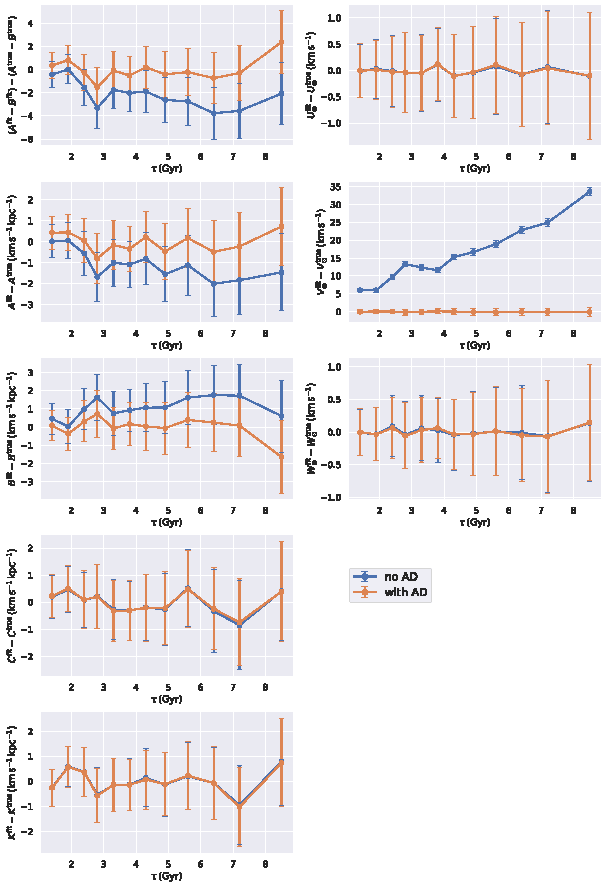
\includegraphics[width=15cm]{fig/Mock_AD.pdf}
	\caption{解析1。1000個の星の模擬データをasymmetric drift有り、無しで解析した結果。左図は各パラメータの解析結果。縦軸は各パラメータの値、横軸は模擬データに入れた速度分散に対応する年齢。trueは設定値、no ADはasymmetric driftを考慮していない解析結果、with ADはasymmetric driftを考慮した解析結果であることを示している。左側の図は各パラメータごとの値。右側上図は相対誤差、右側下図は絶対誤差を表している。} \label{fig:Mock_AD}
\end{figure*}

%%%%%%%%%%%%%%%%%%%%%%%%%%%%%%%%%%%%%%%%%%%%%%%%%%%%%%%%%%%%%%%%%%%%%%%%%%%%%%%%%%%%%%%%%%%%%%%%
%%%%%%%%%%%%%%%%%%%%%%%%%%%%%%%%%%%%%%%%%%%%%%%%%%%%%%%%%%%%%%%%%%%%%%%%%%%%%%%%%%%%%%%%%%%%%%%%
%%%%%%%%%%%%%%%%%%%%%%%%%%%%%%%%%%%%%%%%%%%%%%%%%%%%%%%%%%%%%%%%%%%%%%%%%%%%%%%%%%%%%%%%%%%%%%%%

\subsection{解析2: 視線速度の有無による解析結果への影響}
解析2では、asymmetric driftを入れずに模擬データを生成し、それを視線速度を含めた尤度関数式(\ref{Likelihood_Mock})と含めない尤度関数
\begin{align}
\begin{aligned}
	\ln \mathcal{L} =& -\frac{1}{2}\sum_i \left(\frac{\left[\mu_{l,i} - \mu_l^{\mathrm{OL}}(l_i,b_i,\varpi_i)\right]^2}{\sigma_{\mu_l}^2 + (s_{\mu_{l,i}})^2}  + {\rm ln}\left[\sigma_{\mu_l}^2 + (s_{\mu_{l,i}})^2\right] \right. \\
	&+ \left. \frac{\left[\mu_{b,i} - \mu_b^{\mathrm{OL}}(l_i,b_i,\varpi_i)\right]^2}{\sigma_{\mu_b}^2 + (s_{\mu_{b,i}})^2}  + {\rm ln}\left[\sigma_{\mu_b}^2 + (s_{\mu_{b,i}})^2\right] \right)
\end{aligned}
\end{align}
とで解析した。各パラメータの値は表\ref{table4}を用いている。asymmetric driftは模擬データ生成でも解析でも考慮していない。視線速度を含めた観測方程式(\ref{ObsEq})での解析と含めない解析との結果を比較する(\ref{fig:Mock_vlos})。右側の図を見ると、$B$だけは速度分散無しの解析の方が有りの解析よりも少し良い精度となっているが、それ以外のパラメータでは視線速度有りの方が数\%程度高い精度となっている。

\begin{figure*}[htbp]
	\centering
	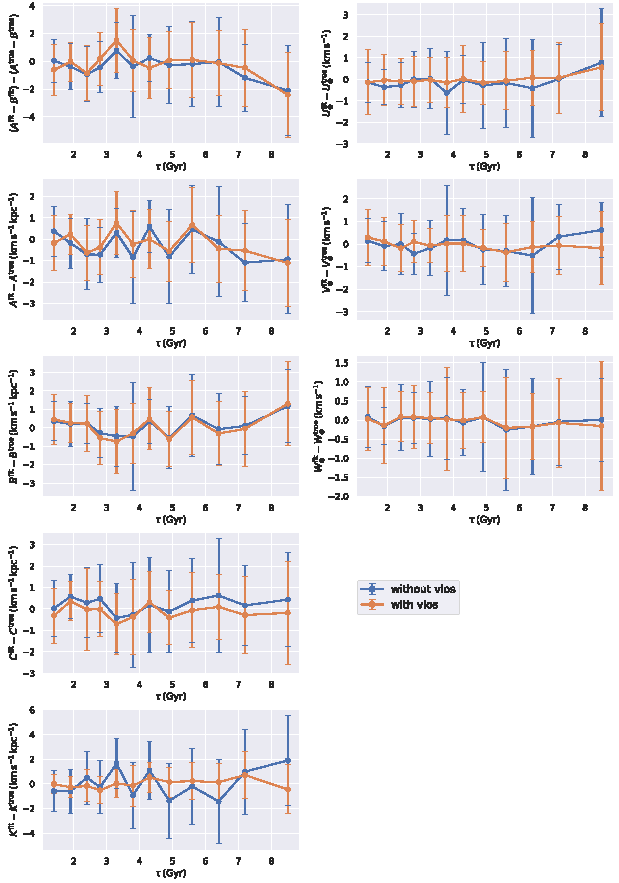
\includegraphics[width=15cm]{fig/Mock_vlos.pdf}
	\caption{解析2。視線速度の観測方程式有りと無しで解析したときの結果の絶対誤差、相対誤差と相対誤差のlogスケール。横軸は各パラメータとなっている。視線速度有りの解析の方が無しの解析よりも精度が高いことがわかる。左側の図は各パラメータごとの値。右側上図は相対誤差、右側下図は絶対誤差を表している。} \label{fig:Mock_vlos}
\end{figure*}

%%%%%%%%%%%%%%%%%%%%%%%%%%%%%%%%%%%%%%%%%%%%%%%%%%%%%%%%%%%%%%%%%%%%%%%%%%%%%%%%%%%%%%%%%%%%%%%%
%%%%%%%%%%%%%%%%%%%%%%%%%%%%%%%%%%%%%%%%%%%%%%%%%%%%%%%%%%%%%%%%%%%%%%%%%%%%%%%%%%%%%%%%%%%%%%%%
%%%%%%%%%%%%%%%%%%%%%%%%%%%%%%%%%%%%%%%%%%%%%%%%%%%%%%%%%%%%%%%%%%%%%%%%%%%%%%%%%%%%%%%%%%%%%%%%

\subsection{解析3: 速度楕円体の傾きの解析結果への影響 \label{解析3}}
速度楕円体を傾けた模擬データを5パターン生成し、それぞれを同じ方法で解析した。5パターンというのは、速度楕円体の傾き$0、10、20、30、40^{\circ}$の5パターンの傾け方をしているためである。具体的には、速度$v_R$と$v_{\phi}$の間の速度楕円体の傾きを$l_{R\phi}$するとき、
\begin{align}
\begin{aligned}
	\left(
	\begin{array}{c}
	 	\sigma_{R,\mathrm{VE}}\\
	 	\sigma_{\phi,\mathrm{VE}}
	\end{array}
	\right)
	=
	\left(
	\begin{array}{cc}
	 	\cos{l_{R\phi}} & -\sin{l_{R\phi}}\\
	 	\sin{l_{R\phi}} & -\cos{l_{R\phi}}
	\end{array}
	\right)
	\left(
	\begin{array}{c}
	 	\sigma_R\\
	 	\sigma_{\phi}
	\end{array}
	\right)
\end{aligned}
\end{align}
のように$\sigma_R、\sigma_{\phi}$で描かれる速度楕円体を$l_{R\phi}$だけ回転させている。

図\ref{fig:Mock_VE}は速度楕円体の傾き$l_{R\phi}$を$0,10,20,30,40$度の5通りに設定した模擬データを生成し、それらをそれぞれ解析した結果である。この解析での試行回数は10回であり、10回の解析結果の値の平均値を図\ref{fig:Mock_VE}にプロットしている。また、この解析ではasymmetric driftは考慮していない。この結果では$l_{R\phi}$の値による大きな違いは見られなかった。

\begin{figure*}[htbp]
	\centering
	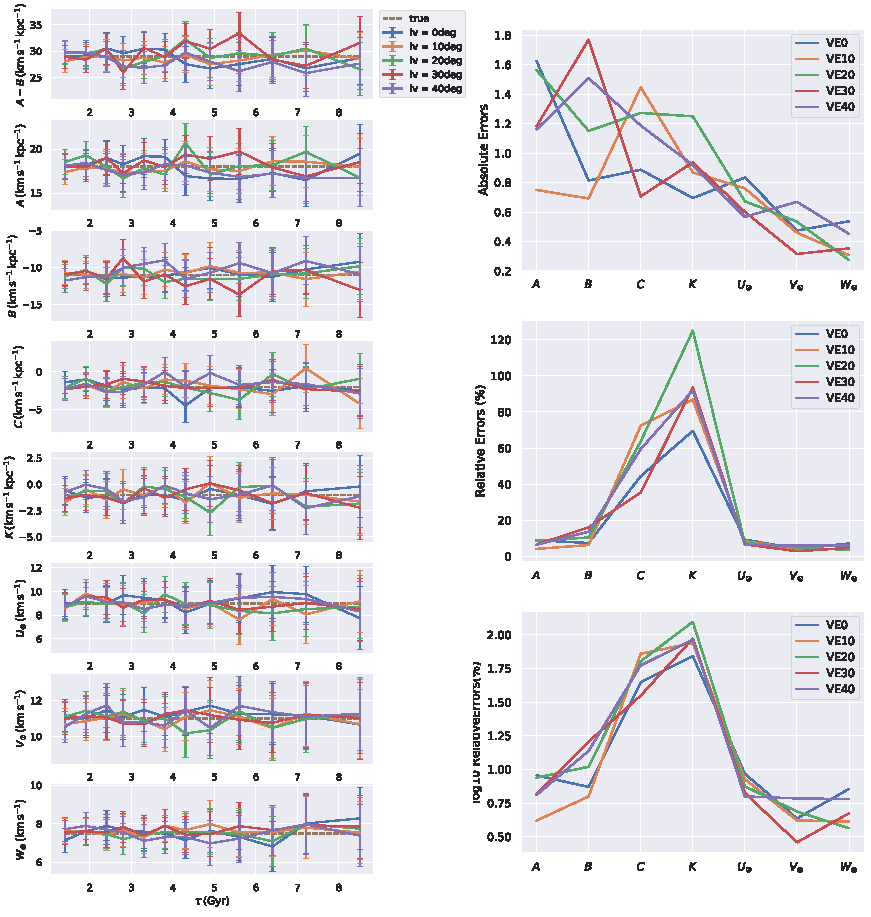
\includegraphics[width=15cm]{fig/Mock_VE.pdf}
	\caption{解析3。1000個の星の模擬データを速度楕円体の傾き$0,10,20,30,40$度で解析した結果。縦軸は各パラメータの値、横軸は模擬データに入れた速度分散に対応する年齢。左側の図は各パラメータごとの値。右側上図は相対誤差、右側下図は絶対誤差を表している。} \label{fig:Mock_VE}
\end{figure*}


%%%%%%%%%%%%%%%%%%%%%%%%%%%%%%%%%%%%%%%%%%%%%%%%%%%%%%%%%%%%%%%%%%%%%%%%%%%%%%%%%%%%%%%%%%%%%%%%
%%%%%%%%%%%%%%%%%%%%%%%%%%%%%%%%%%%%%%%%%%%%%%%%%%%%%%%%%%%%%%%%%%%%%%%%%%%%%%%%%%%%%%%%%%%%%%%%
%%%%%%%%%%%%%%%%%%%%%%%%%%%%%%%%%%%%%%%%%%%%%%%%%%%%%%%%%%%%%%%%%%%%%%%%%%%%%%%%%%%%%%%%%%%%%%%%

\subsection{解析4: 太陽からの距離の解析結果への影響}
解析4では、表\ref{table4}で用いている値を仮定した上で、太陽からの距離$D$の範囲を$D<\SI{300}{pc}、\SI{400}{pc}、\SI{500}{pc}、\SI{600}{pc}、\SI{700}{pc}、\SI{800}{pc}、\SI{900}{pc}、\SI{1}{kpc}$のように変えてデータを生成している。つまり、例えば$D<\SI{300}{pc}$の場合には、太陽からの距離$\SI{300}{pc}$までの中で1000個の星の位置・速度データを生成するということである。そうして生成した模擬データをそれぞれ解析し、解析結果の平均値を図\ref{fig:Mock_D}にプロットしている。得られた確率分布の標準偏差も平均値を使用している。

$D<0.3\,\mathrm{kpc}$ではオールト定数$A、B、C、K$が他のパターンに比べて精度が悪い。他の距離の範囲でも、パラメータによるが$D$が大きいほど精度が高い傾向がある。しかし、この差は決して大きい差ではなく、$D=\SI{400}{pc}$より広範囲であればあまり差はないと考えられる。

\begin{figure*}[htbp]
	\centering
	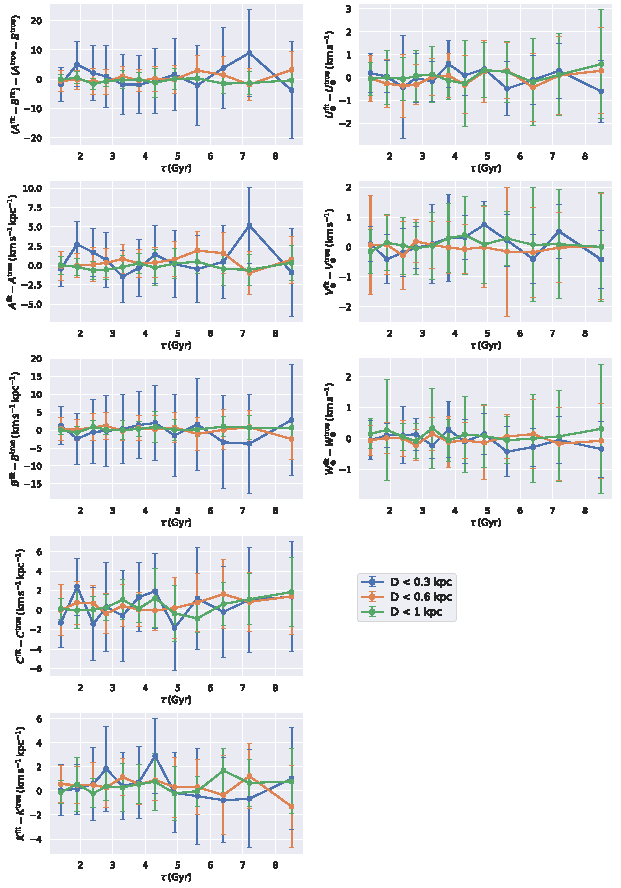
\includegraphics[width=15cm]{fig/Mock_D.pdf}
	\caption{解析4。1000個の星の模擬データを太陽からの距離$D<0.3、0.4、0.5、0.6、0.7、0.8、0.9、1\  \mathrm{kpc}$の8パターンで生成し、解析した結果。つまり、例えば$D<\SI{0.3}{kpc}$のときには太陽からの距離$\SI{0.3}{kpc}$の内部に星1000個を生成し、それを解析した結果が$D<\SI{0.3}{kpc}$の解析結果ということである。縦軸は各パラメータの値、横軸は模擬データに入れた速度分散に対応する年齢。左側の図は各パラメータごとの値。右側上図は相対誤差、右側下図は絶対誤差を表している。ラベルのD03は$D<0.3\,\mathrm{kpc}$、D04は$D<0.4\,\mathrm{kpc}$を意味する。} \label{fig:Mock_D}
\end{figure*}

%%%%%%%%%%%%%%%%%%%%%%%%%%%%%%%%%%%%%%%%%%%%%%%%%%%%%%%%%%%%%%%%%%%%%%%%%%%%%%%%%%%%%%%%%%%%%%%%
%%%%%%%%%%%%%%%%%%%%%%%%%%%%%%%%%%%%%%%%%%%%%%%%%%%%%%%%%%%%%%%%%%%%%%%%%%%%%%%%%%%%%%%%%%%%%%%%
%%%%%%%%%%%%%%%%%%%%%%%%%%%%%%%%%%%%%%%%%%%%%%%%%%%%%%%%%%%%%%%%%%%%%%%%%%%%%%%%%%%%%%%%%%%%%%%%

\subsection{解析5: 円盤面からの距離の解析結果への影響}
解析5では各パラメータの値は表\ref{table4}を用いている。asymemtric driftは模擬データにも解析にも考慮していない。図\ref{fig:Mock_z}はサンプル星の円盤面からの距離$|z|$の範囲を変えて生成した模擬データの解析結果である。つまり、$|z|=100\,\mathrm{pc}$の場合、円盤面から$100\,\mathrm{pc}$以内に星を1000個生成し、それぞれに星にOort-Lindbladモデルに従う速度を持たせ、それに観測方程式(\ref{ObsEq})を当てはめる形で解析している。。この解析結果からは$|z|$の値による大きな違いは見られず、わずかな値の違いはランダム性によるものだと考えられる。

\begin{figure*}[htbp]
	\centering
	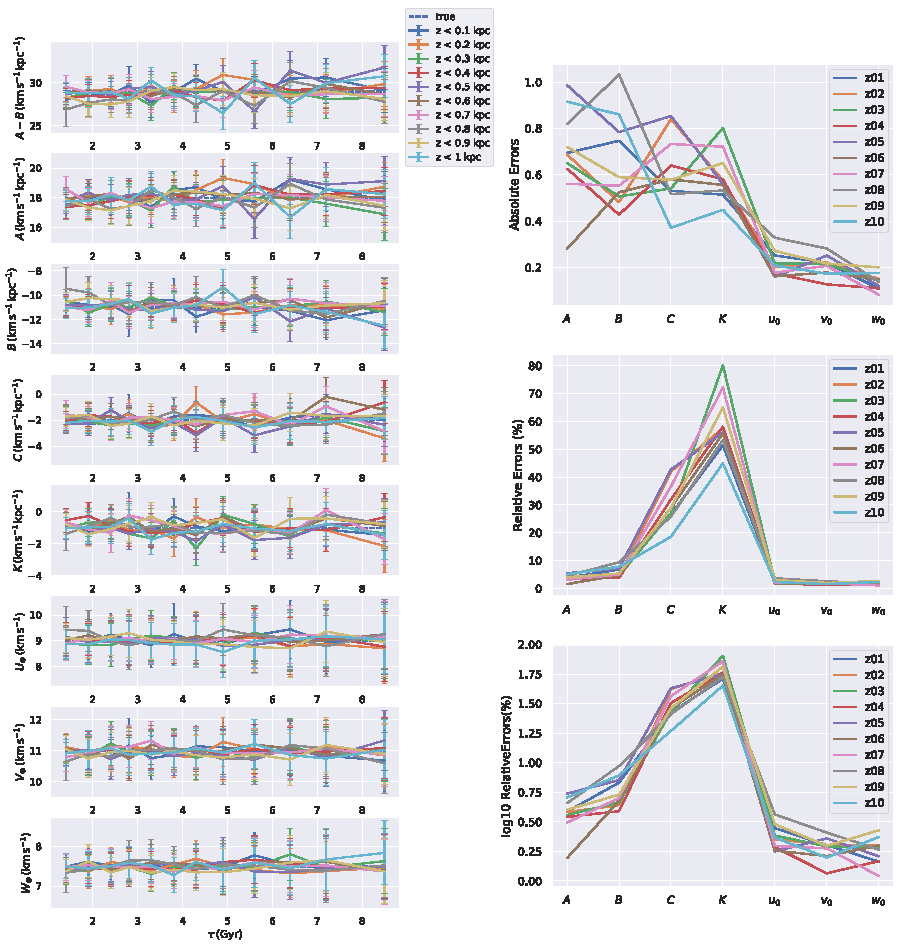
\includegraphics[width=15cm]{fig/Mock_z.pdf}
	\caption{解析5。1000個の星の模擬データを円盤面からの距離の範囲を$|z|<0.1、0.2、0.3、0.4、0.5、0.6、0.7、0.8、0.9、1\,\mathrm{kpc}$と変えて解析した結果。縦軸は各パラメータの値、横軸は模擬データに入れた速度分散に対応する年齢。左側の図は各パラメータごとの値。右側上図は相対誤差、右側下図は絶対誤差を表している。} \label{fig:Mock_z}
\end{figure*}

%%%%%%%%%%%%%%%%%%%%%%%%%%%%%%%%%%%%%%%%%%%%%%%%%%%%%%%%%%%%%%%%%%%%%%%%%%%%%%%%%%%%%%%%%%%%%%%%
%%%%%%%%%%%%%%%%%%%%%%%%%%%%%%%%%%%%%%%%%%%%%%%%%%%%%%%%%%%%%%%%%%%%%%%%%%%%%%%%%%%%%%%%%%%%%%%%
%%%%%%%%%%%%%%%%%%%%%%%%%%%%%%%%%%%%%%%%%%%%%%%%%%%%%%%%%%%%%%%%%%%%%%%%%%%%%%%%%%%%%%%%%%%%%%%%

\subsection{解析6:サンプル数の解析結果への影響 \label{new_N}}
模擬データを生成する際に乱数を発生させているため、サンプル数が少なすぎるとポアソンノイズが解析結果に効いてしまうと考えられる。サンプル数の解析結果への影響を調べる上では、ポアソンノイズによる差をできるだけ排除する必要がある。そこで、サンプル数の合計値が10万になるように試行回数を調整をした。つまり、サンプル数100のときは試行回数1000、サンプル数1000のときは試行回数100としている。
\begin{figure*}[htbp]
	\centering
	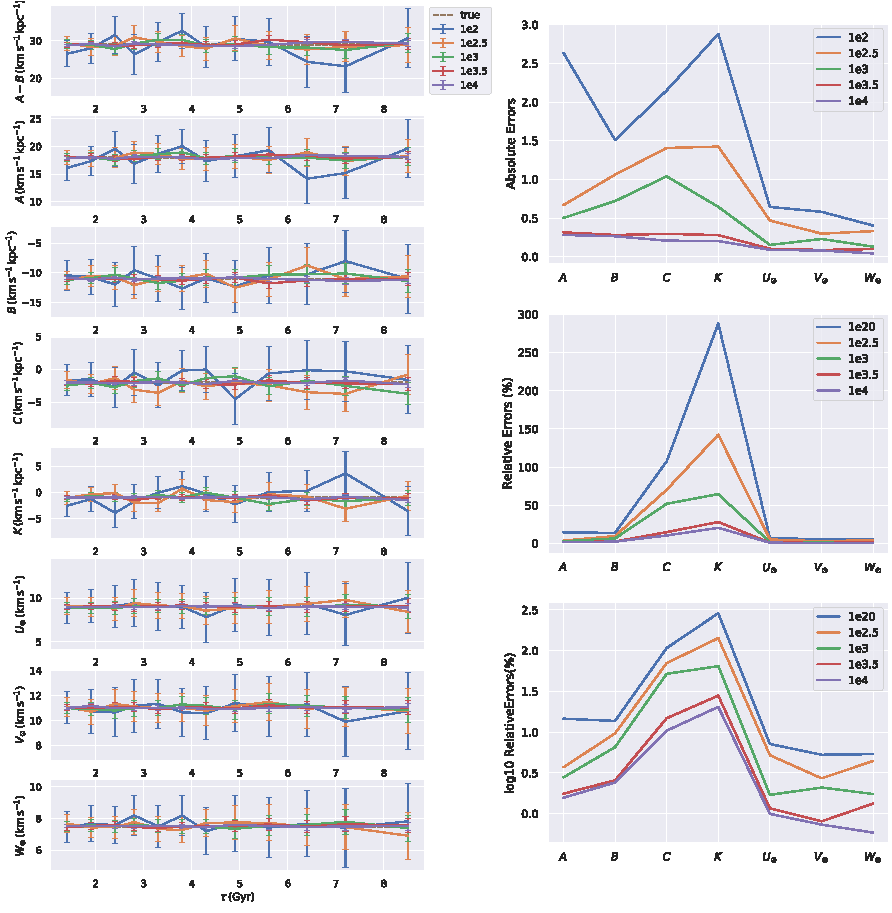
\includegraphics[width=15cm]{fig/Mock_N.pdf}
	\caption{解析6。サンプル数を変えて解析したときの結果の相対誤差。横軸は各パラメータ、縦軸は模擬データ生成時に設定した値と解析結果の値との相対誤差のlogスケール。サンプル数が多いほど相対誤差が小さくなっていることがわかる。左側の図は各パラメータごとの値。右側上図は相対誤差、右側下図は絶対誤差を表している。} \label{fig:Mock_N}
\end{figure*}

%%%%%%%%%%%%%%%%%%%%%%%%%%%%%%%%%%%%%%%%%%%%%%%%%%%%%%%%%%%%%%%%%%%%%%%%%%%%%%%%%%%%%%%%%%%%%%%%
%%%%%%%%%%%%%%%%%%%%%%%%%%%%%%%%%%%%%%%%%%%%%%%%%%%%%%%%%%%%%%%%%%%%%%%%%%%%%%%%%%%%%%%%%%%%%%%%
%%%%%%%%%%%%%%%%%%%%%%%%%%%%%%%%%%%%%%%%%%%%%%%%%%%%%%%%%%%%%%%%%%%%%%%%%%%%%%%%%%%%%%%%%%%%%%%%

\subsection{解析7: $R_{\odot}$の値の解析結果への影響}
オールト定数と太陽運動の測定の先行研究では、仮定されている太陽と銀河中心との距離$R_{\odot}$がそれぞれの先行研究で異なる。この値はだいたい$\SI{7.5}{kpc}$から$\SI{8.5}{kpc}$の間であり、最大約10\%の違いがある。そこで、仮定する$R_{\odot}$の値が実際の$R_{\odot}$と異なる場合にどの程度測定値を間違うのかを調べることにした。

解析7では、表\ref{table4}のパラメータ値を仮定して模擬データを生成し、$R_{\odot}$の値を$R_{\odot} = 6、6.4、6.8、7.2、7.6、8.0、8.4、8.8、9.2、9.6、10\,\si{kpc}$と変えて11パターンで解析した。asymmetric driftは模擬データでも解析でも考慮している。なぜなら、$R_{\odot}$はasymmetric driftを考慮するときのみ使用するからである。具体的には式(\ref{eq142})の上から2つ目の式と式(\ref{eq153})で$R_{\odot}$を使用する。図\ref{fig:Mock_R0}は解析7の結果である。この図を見ると、オールト定数$A、B$は他のパラメータに比べ大きく間違った値となっている。右側上図の相対誤差では、模擬データで設定している値と同じ$R_{\odot}=\SI{8.2}{kpc}$のときの相対誤差が最も小さく、$R_{\odot}$の値が$\SI{8.2}{kpc}$から離れるほど相対誤差が大きくなっていることが分かる。右側下図の絶対誤差を見ると、$A、B、U_{\odot}、V_{\odot}、W_{\odot}$が解析で仮定する$R_{\odot}$によって異っていることが分かる。しかし、仮定する$R_{\odot}$への依存性は確認できない。

\begin{figure*}[htbp]
	\centering
	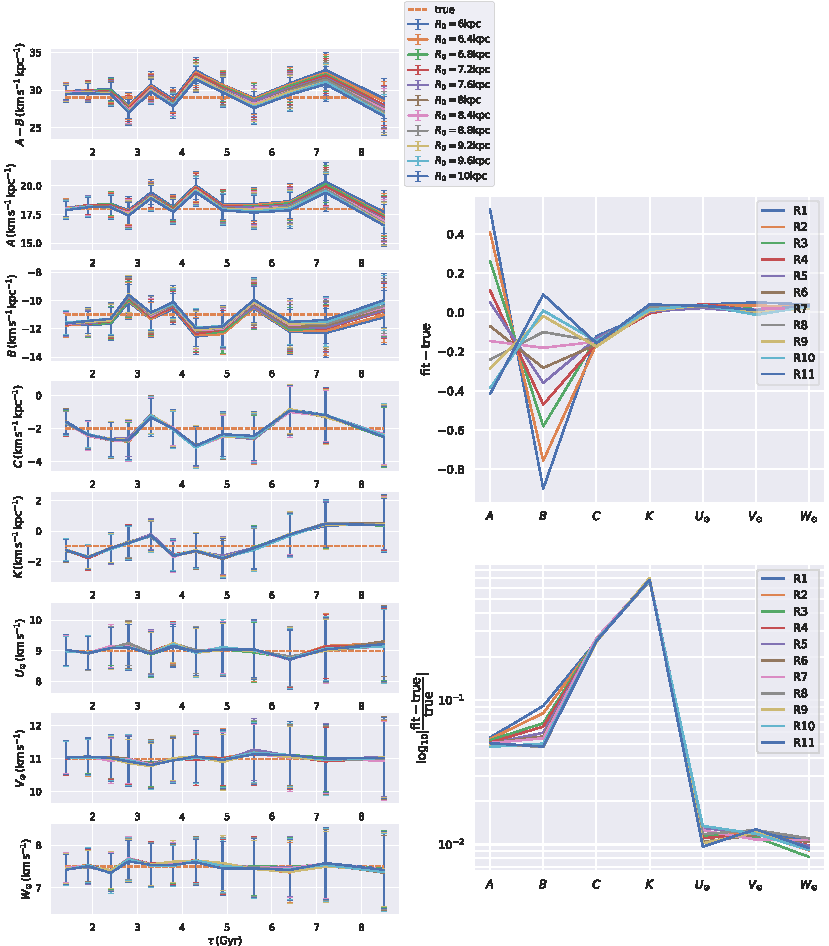
\includegraphics[width=15cm]{fig/Mock_R0.pdf}
	\caption{解析7。1000個の星の模擬データを太陽の銀河中心からの距離$R_{\odot}$を$R_{\odot} = 6、6.4、6.8、7.2、7.6、8.0、8.4、8.8、9.2、9.6、10\,\si{kpc}$と変えて解析した結果。ラベルのR1は$R_{\odot}=6\,\si{kpc}$、R2は$R_{\odot}=6.4\,\si{kpc}$に対応している。縦軸は各パラメータの値、横軸は模擬データに入れた速度分散に対応する年齢。左側の図は各パラメータごとの値。右側上図は相対誤差、右側下図は絶対誤差を表している。} \label{fig:Mock_R0}
\end{figure*}